\chapter{Galois群与Kronecker--Weber定理}\label{L1}
\lecturedate{2020/02/17}
\sourcepage{3}
Langlands纲领起源于数论，其开端是对Galois扩张$L/F$的Galois群$\Gal(L/F)$的研究。
\section{基本定义与性质}\label{L1S1}
设$F$为任意域，$L$为$F$的一个扩张。
\begin{definition*}{有限扩张}\idx{有限扩张}
如果$L$作为$F$-向量空间是有限维的，就称$L/F$为\textbf{有限扩张}。称$\dim_F L$为$L$在$F$上的\textbf{次数}，记作$[L:F]$。
\end{definition*}
\begin{definition*}{代数扩张}\idx{代数扩张}
$L/F$是\textbf{代数扩张}$\iff L$中的每个元素都是$F[x]$中某个非零多项式的根$\iff L/F$是有限子扩张的并。
\end{definition*}
\begin{definition*}{正规扩张}\idx{正规扩张}
如果$L/F$是代数扩张，且$F[x]$中每个在$L$中有一个根的不可约多项式，其所有根都在$L$中，就称$L/F$为\textbf{正规扩张}。
\end{definition*}
\begin{property}每个代数扩张都有正规闭包。\end{property}
\begin{definition*}{可分扩张}\idx{可分扩张}
如果$L/F$是代数扩张，且$L$中每个元素在$F$上的极小多项式在$F$的代数闭包中都没有重根，就称$L/F$为\textbf{可分扩张}。
\end{definition*}
\begin{property}由本原元定理，每个有限可分扩张$L/F$都有一个本原元，即$L=F(\alpha)$，其中$\alpha$在$F$上是代数的。\end{property}
\sourcepage{4}
\begin{property}如果$\operatorname{char}(F)=0$，或$F$为有限域，那么每个代数扩张$L/F$都是可分的。（这是因为在这些情形中，$F$都是完美域\znote{域 $F$ 称为\textbf{完美域}（perfect field），若 $F$ 上每个不可约多项式都无重根；特征 $p>0$ 时这等价于 $F^p=F$，即 Frobenius 映射 $x\mapsto x^p$ 是满射。完美域的代数闭包与其可分闭包重合，因此它的每个代数扩张都自动可分，这正解释了本条结论。[来源：nLab "perfect field"，\url{https://ncatlab.org/nlab/show/perfect+field}（Last revised 2017-07-21；2026-11-14 访问）。]}。）\end{property}
\begin{definition*}{Galois扩张与Galois群}\idx{Galois扩张}\idx{Galois群}
如果$L/F$既正规又可分，就称它为\textbf{Galois扩张}。\textbf{Galois群}$\Gal(L/F)$是由$L$中所有逐点固定$F$的自同构组成的群。
\end{definition*}
\begin{property}
\begin{itemize}
\item 若$L/F$是有限Galois扩张，则$|\Gal(L/F)|=[L:F]$。
\item $L/F$是有限Galois扩张$\iff L$是$F[x]$中某个可分多项式的分裂域。
\item 如果$F$是完美域（例如$\operatorname{char}(F)=0$或$F$是有限域），那么$F$的代数闭包$\overline F$就是$F$的最大Galois扩张。
\item Galois理论基本定理指出：若$L/F$是Galois扩张，则$F=L^{\Gal(L/F)}$；对于$L$中每个包含$F$的子域$K$，$L/K$都是Galois扩张，而且映射
\[
\{K\mid F\subseteq K\subseteq L\}\longrightarrow\{H\mid H\subseteq\Gal(L/F)\},\qquad K\longmapsto\Gal(L/K)
\]
是单射；当$L/F$有限时，它给出一个反向包含的双射。此外，$\Gal(L/K)$是$\Gal(L/F)$的正规子群，当且仅当$K/F$为Galois扩张，此时有群的正合列
\[1\longrightarrow\Gal(L/K)\longrightarrow\Gal(L/F)\longrightarrow\Gal(K/F)\longrightarrow1.\]
\item 如果$L/F$是无限Galois扩张，就在$\Gal(L/F)$上定义一种称为\textbf{Krull拓扑}的拓扑，从而得到中间域与$\Gal(L/F)$的闭子群之间的双射。（见本讲末尾的\hyperref[L1S3]{参考文献}。）\idx{Krull拓扑}\znote{具体地，把 $\Gal(L/F)$ 看作所有有限 Galois 子扩张 $L_i/F$ 对应的有限群 $\Gal(L_i/F)$ 的投影极限，并赋以投影极限拓扑（各 $\Gal(L_i/F)$ 取离散拓扑），所得拓扑即 Krull 拓扑。此时 $\Gal(L/F)$ 是\textbf{射有限群}：紧、Hausdorff、全不连通。正因如此，才对「闭子群」而非任意子群有中间域对应——非闭子群不对应任何中间域。[来源：nLab "profinite group"，\url{https://ncatlab.org/nlab/show/profinite+group}（Last revised 2025-07-01；2026-11-14 访问）。]}
\end{itemize}
\end{property}
\begin{definition*}{阿贝尔扩张}\idx{阿贝尔扩张}
如果$L/F$是Galois扩张，且$\Gal(L/F)$为阿贝尔群，就称$L/F$为\textbf{阿贝尔扩张}。
\end{definition*}
\begin{property}若$L/F$是阿贝尔扩张，则$L$中每个包含$F$的子域$K$都是$F$的阿贝尔扩张。这是因为阿贝尔群的每个子群都是正规子群，而且阿贝尔群的每个商群也都是阿贝尔群。\end{property}
\sourcepage{5}
从现在起，我们总用$\overline F$表示域$F$的可分闭包\znote{\textbf{可分闭包} $F^{\mathrm{sep}}$ 指 $\overline F_{\mathrm{alg}}$ 中所有在 $F$ 上可分的元素组成的子域（本文记作 $\overline F$）。它是 $F$ 的极大可分扩张，故 $F^{\mathrm{sep}}/F$ 是 Galois 扩张；$F$ 完美时它与代数闭包重合。数论中取可分闭包而非代数闭包作底座，是因为 $\Gal(F^{\mathrm{sep}}/F)$ 才是与类域论、Langlands 对应直接相关的绝对 Galois 群。[来源：nLab "separable closure"，\url{https://ncatlab.org/nlab/show/separable+closure}（Last revised 2026-04-15；2026-11-14 访问）。]}，它也是$F$的最大Galois扩张。当$F$是完美域时，$\overline F$也就是$F$的代数闭包。由Galois理论基本定理，$F$的每个Galois扩张都可由$\Gal(\overline F/F)$的一个闭正规子群确定。因此，数论中的一个主要问题就是描述$\Gal(\overline F/F)$。
\originalnumber{1}
\begin{example}\label{L1S1O1}
设$F=\R$，则$\Gal(\overline F/F)=\Gal(\C/\R)=\{1,\sigma\}$，其中$\sigma:\C\xrightarrow{\sim}\C$把每个复数映到它的共轭复数。$\C/\R$是阿贝尔扩张；由于$\Gal(\C/\R)$没有非平凡的真子群，$\R$没有其他非平凡的Galois扩张。
\end{example}
\originalnumber{2}
\begin{example}\label{L1S1O2}
设$F=\Q$，$L$为二次数域（即$[L:\Q]=2$）。每个二次数域都形如$\Q(\sqrt d)$，其中$d$为无平方因子的整数，因此$L/\Q$是Galois扩张，且$\Gal(L/\Q)=\{1,\sigma\}$，其中$\sigma(\sqrt d)=-\sqrt d$。
\end{example}
下面列出两个命题供以后使用，证明从略。
\originalnumber{3}
\begin{proposition}\label{L1S1O3}
\begin{enumerate}
\item 若$L_1/F$与$L_2/F$都是阿贝尔扩张，且$L_1,L_2$是某个共同域的子域，则合成域$L_1L_2$在$F$上也是阿贝尔扩张。
\item $L/F$是阿贝尔扩张$\iff L/F$是有限阿贝尔子扩张的并。
\end{enumerate}
\end{proposition}
注意，若$L/F$是阿贝尔扩张，则$L=\bigcup_{\alpha\in L}F(\alpha)$，且每个$F(\alpha)/F$都是阿贝尔扩张。
\originalnumber{4}
\begin{proposition}\label{L1S1O4}
设$L_1,L_2$是$F$的两个Galois扩张，并假定它们是某个共同域的子域。那么$L_1L_2/F$也是Galois扩张，且映射
\[\Gal(L_1L_2/F)\longrightarrow\Gal(L_1/F)\times\Gal(L_2/F)\]
是单射。若$L_1\cap L_2=F$，则这个映射是同构。
\end{proposition}
\section{\texorpdfstring{$\Q$的Galois扩张}{Q的Galois扩张}}\label{L1S2}
设$F$为代数数域，即$F/\Q$是有限扩张。一般而言，我们对$\Gal(\overline F/F)$了解得还不多。
\sourcepage{6}
Langlands纲领建议人们研究$\Gal(\overline F/F)$的所有$n$维表示，而不是直接研究这个群本身的结构。Robert Langlands提出的优美猜想，实际上是对$n=1$情形的推广；$n=1$的结论已由类域论证明。

先来看$n=1$的情形。注意，对于任意群$G$，它的一维表示与其最大阿贝尔商群的一维表示相同；这里的最大阿贝尔商群，是以交换子生成的闭正规子群为核得到的商群。\znote{即\textbf{阿贝尔化} $G^{\mathrm{ab}}=G/\overline{[G,G]}$：一般群取交换子子群的闭包，使商群 Hausdorff（射有限情形下闭包不可省）。$G$ 的一维表示与 $G^{\mathrm{ab}}$ 的一维表示一一对应，而无限 Galois 理论给出 $\Gal(\overline F/F)^{\mathrm{ab}}\cong\Gal(F^{\mathrm{ab}}/F)$，所以 $n=1$ 的 Langlands 对应就是描述 $F^{\mathrm{ab}}$。$n\geq2$ 的表示没有这种「先取商」的化简，这正是难点所在。[来源：nLab "abelianization"，\url{https://ncatlab.org/nlab/show/abelianization}（Last revised 2026-01-21；2026-11-14 访问）。]}此外，考察一维表示便能确定这个阿贝尔群。因此，在$n=1$时，我们要做的是描述$\Gal(\overline F/F)$的最大阿贝尔商群。由无限Galois理论基本定理，存在一个最大阿贝尔扩张$F^{\mathrm{ab}}$，且$\Gal(F^{\mathrm{ab}}/F)$就是$\Gal(\overline F/F)$的最大阿贝尔商群。

本节将明确描述$\Q^{\mathrm{ab}}$和$\Gal(\Q^{\mathrm{ab}}/\Q)$。首先介绍一类典型的$\Q$的有限Galois扩张。
\originalnumber{1}
\begin{definition}{分圆域}\label{L1S2O1}\idx{分圆域}
设$m$为正整数，$\zeta_m=e^{2\pi i/m}$。则$\Q(\zeta_m)$是$x^m-1$的分裂域\znote{设 $f\in F[x]$。$f$ 在 $F$ 上的\textbf{分裂域}指这样的扩张 $E/F$：$f$ 在 $E$ 中分裂为一次因式之积，且 $E$ 由 $F$ 与 $f$ 的全部根生成；它在 $F$-同构意义下唯一。$x^m-1$ 的根恰为全部 $m$ 次单位根，故其分裂域为 $\Q(\zeta_m)$。[来源：nLab "splitting field"，\url{https://ncatlab.org/nlab/show/splitting+field}（Last revised 2026-06-08；2026-11-14 访问）。]}，称为由$m$次单位根生成的\textbf{分圆域}。
\end{definition}
\originalnumber{2}
\begin{proposition}\label{L1S2O2}
$\Gal(\Q(\zeta_m)/\Q)\cong(\Z/m\Z)^\times$。
\end{proposition}
\begin{proof}
定义群同态$\theta:\Gal(\Q(\zeta_m)/\Q)\longrightarrow(\Z/m\Z)^\times$，使得对每个$\sigma\in\Gal(\Q(\zeta_m)/\Q)$，有$\sigma(\zeta_m)=\zeta_m^{\theta(\sigma)}$。容易看出$\theta$是单射，且像为整个$(\Z/m\Z)^\times$。
% [Tutor Note: 原书 p6 将 $\theta$ 的余域写作 $\Z/m\Z$，紧接着又说其像为 $(\Z/m\Z)^\times$，前后不一致；译文按正确的 $(\Z/m\Z)^\times$ 处理。]
\end{proof}
\originalnumber{3}
\begin{note}[L1S2O3]
容易看出，若$m\mid n$，则$\Q(\zeta_m)\subseteq\Q(\zeta_n)$；由Galois理论，$\Gal(\Q(\zeta_m)/\Q)$是$\Gal(\Q(\zeta_n)/\Q)$的商群。下面的图表交换：
\begin{figure}[H]\centering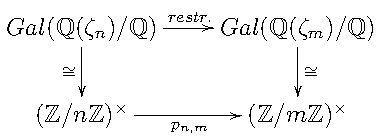
\includegraphics[width=0.3057\paperwidth]{images/L1-p006-diagram.pdf}\end{figure}
其中$p_{n,m}$把$[a]$映到$a\bmod m$。
\end{note}
\sourcepage{7}
对任意正整数$m$，定义$\varphi(m)$为$1$到$m$之间与$m$互素的整数个数。于是
\[|\Gal(\Q(\zeta_m)/\Q)|=[\Q(\zeta_m):\Q]=|(\Z/m\Z)^\times|=\varphi(m).\]
在经典数论中，算术函数$\varphi$称为\textbf{Euler函数}，并有如下结论。\idx{Euler函数}
\originalnumber{4}
\begin{theorem}\label{L1S2O4}
若$n=p_1^{a_1}\cdots p_l^{a_l}$，其中$p_1,\ldots,p_l$是$\Z$中互不相同的素数，则
\[\varphi(n)=n\left(1-\frac1{p_1}\right)\cdots\left(1-\frac1{p_l}\right).\]
\end{theorem}
\eref{定理}{L1S2O4}的证明从略，本讲末尾将给出参考文献。
\originalnumber{5}
\begin{corollary}\label{L1S2O5}
设$m,n$为两个互素的正整数，则$\Q(\zeta_n,\zeta_m)=\Q(\zeta_{mn})$。此外，$\Q(\zeta_m)\cap\Q(\zeta_n)=\Q$，因而由\eref{命题}{L1S1O4}，
\[\Gal(\Q(\zeta_{mn})/\Q)\cong\Gal(\Q(\zeta_m)/\Q)\times\Gal(\Q(\zeta_n)/\Q).\]
\end{corollary}
\begin{proof}
由$\zeta_{mn}^{m}=\zeta_n$和$\zeta_{mn}^{n}=\zeta_m$，有$\Q(\zeta_m,\zeta_n)\subseteq\Q(\zeta_{mn})$。另一方面，因$(m,n)=1$，存在整数$u,v$使$vm+un=1$。于是$\zeta_n^v\zeta_m^u=\zeta_{mn}$，故$\Q(\zeta_{mn})\subseteq\Q(\zeta_m,\zeta_n)$。

为证明$\Q(\zeta_m)\cap\Q(\zeta_n)=\Q$，只需证明$[\Q(\zeta_m,\zeta_n):\Q]=[\Q(\zeta_m):\Q]\,[\Q(\zeta_n):\Q]$。
% [Tutor Note: 原书 p7 该恒等式右端误写作 $[\Q(\zeta_n):\Q]\cdot[\Q(\zeta_n):\Q]$（两次 $\zeta_n$）；译文按正确写法处理。]因此，证明$\varphi(mn)=\varphi(m)\varphi(n)$即可。写成$n=p_1^{a_1}\cdots p_l^{a_l}$、$m=p_{l+1}^{a_{l+1}}\cdots p_{l+t}^{a_{l+t}}$，其中$p_1,\ldots,p_{l+t}$互不相同；由\eref{定理}{L1S2O4}，
\[\varphi(mn)=mn\left(1-\frac1{p_1}\right)\cdots\left(1-\frac1{p_{l+t}}\right)=\varphi(m)\varphi(n).\]
\end{proof}
在介绍Kronecker--Weber定理之前，我们稍作离题，先给出下面这个关于有限阿贝尔Galois群的有趣结论。
\originalnumber{6}
\begin{theorem}\label{L1S2O6}
每个有限阿贝尔群都可以实现为$\Q$的某个阿贝尔扩张的Galois群。
\end{theorem}
\begin{proof}
每个有限阿贝尔群都同构于$\prod_{j=1}^s(\Z/m_j\Z)^{a_j}$，其中$m_j,a_j$为正整数，$m_j$两两不同。
\sourcepage{8}
不失一般性，还可假定$m_j$均为素数的幂。对每个$m_j$，先构造$a_j$个阿贝尔扩张$L_1(m_j),\ldots,L_{a_j}(m_j)$，其Galois群均为$\Z/m_j\Z$。把这些扩张排成一个序列，简记为$L_1,L_2,\ldots$，并要求
\[\left(\prod_{l=1}^{t}L_l\right)\cap L_{t+1}=\Q,\qquad 1\leq t<\sum_{j=1}^s a_j.\]
% [Tutor Note: 原书 p8 此处下界误写作 $1\leq t\leq\sum_j m_j$，与定理中 $m_j$ 的含义不符；译文按正确的 $\sum_j a_j$ 处理。]
这样，由\eref{命题}{L1S1O4}即得所需结论。

从$m_1$开始。选取素数$p_1$使$p_1\equiv1\pmod{m_1}$。于是$\Gal(\Q(\zeta_{p_1})/\Q)$是阶为$p_1-1$的循环群；由于$m_1\mid(p_1-1)$，它有一个阶为$m_1$的子群。
% [Tutor Note: 原书 p8 作 "has a subgroup of order m_1"，旧译误作「指数」；指数为 m_1 的子群对应的是 $\Z/((p_1-1)/m_1)\Z$ 的商，与构造不符。本轮改正。]由Galois理论，得到$\Q(\zeta_{p_1})/\Q$的一个阿贝尔子扩张$L_1(m_1)/\Q$，其Galois群为$\Z/m_1\Z$。为得到$L_2(m_1)$，再选取一个不同于$p_1$的素数$p_2$，满足$p_2\equiv1\pmod{m_1}$，并重复这一过程。由下面的Dirichlet定理，对任意正整数$m$，满足$p\equiv1\pmod m$的素数$p$都有无穷多个。最终得到互不相同的素数$p_1,p_2,\ldots$和阿贝尔扩张$L_1,L_2,\ldots$，其中$L_l\subseteq\Q(\zeta_{p_l})$。由于$\prod_{l=1}^tL_l$包含于$\Q(\zeta_{\prod_{l=1}^t p_l})$，由\eref{推论}{L1S2O5}，
\[\left(\prod_{l=1}^{t}L_l\right)\cap L_{t+1}=\Q,\qquad1\leq t<\sum_{j=1}^s a_j.\]
\end{proof}
\originalnumber{7}
\begin{theorem}{Dirichlet}\label{L1S2O7}\idx{Dirichlet定理}
若$a,b\in\Z$且$(a,b)=1$，$b\ne0$，
% [Tutor Note: 原书 p10 未声明 $b\neq0$，而 $b=0$ 时同余式无意义；译文补上。]则满足$p\equiv a\pmod b$的正素数$p$有无穷多个。
\end{theorem}
\eref{定理}{L1S2O7}的结论曾由Gauss提出猜想，直到1837年才由Dirichlet首次证明。Dirichlet的证明使用了Dirichlet $L$-级数。\znote{Dirichlet $L$-级数定义为 $L(s,\chi)=\sum_{n\geq1}\chi(n)n^{-s}$，其中 $\chi$ 是模 $b$ 的 Dirichlet 特征标；由 $L(1,\chi)\neq0$ 可推出等差数列 $\{a+kb\}$ 中素数无穷多，这就是 Dirichlet 定理的解析证明。它也是 Langlands 纲领中 $L$ 函数的最初原型（$F=\Q$、$n=1$ 的情形）。[来源：K. Ireland, M. Rosen, \textit{A Classical Introduction to Modern Number Theory}, Springer-Verlag New York, 1990, 第 16 章（本讲参考文献 [IM]）；并见 nLab "L-function"，\url{https://ncatlab.org/nlab/show/L-function}（Last revised 2024-07-07；2026-11-14 访问）。]}这里略去证明，稍后给出参考文献。

然而，一旦去掉阿贝尔条件，问题便远未解决。\znote{此即\textbf{逆 Galois 问题}（inverse Galois problem）：是否每个有限群都同构于 $\Q$ 的某个有限 Galois 扩张的 Galois 群？阿贝尔情形由 Kronecker--Weber 定理肯定（即本讲定理 9）；一般情形仍未解决。已知可解群情形成立（Shafarevich），$S_n$、$A_n$ 及大量其他群也已实现，但一般有限群情形是公开问题。[来源：nLab "inverse Galois problem"，\url{https://ncatlab.org/nlab/show/inverse+Galois+problem}（Last revised 2023-05-27；2026-11-14 访问）。]}
\originalnumber{8}
\begin{problem}[（逆Galois问题）]\label{L1S2O8}\idx{逆Galois问题}
每个有限群是否都能实现为$\Q$的某个有限Galois扩张的Galois群？
\end{problem}
分圆域都是$\Q$的阿贝尔扩张，但$\Q$的阿贝尔扩张未必本身就是分圆域，例如二次数域$\Q(\sqrt2)$。
\begin{exercise*}\label{L1S2EX}
证明：二次数域$\Q(\sqrt d)$为分圆域，当且仅当$d=-1$或$-3$。（提示：$[\Q(\sqrt d):\Q]=2$，而$\varphi(m)=2\iff m=3,4,6$。
% [Tutor Note: 原书 p8 习题提示作「$m=4$ 或 $6$」，漏了 $m=3$（$\varphi(3)=2$）；译文已补正。]）
\end{exercise*}
\sourcepage{9}
不过，每个有限阿贝尔扩张都是某个分圆域的子域，正如下面这个优美定理所述。
\originalnumber{9}
\begin{theorem}{Kronecker--Weber}\label{L1S2O9}\idx{Kronecker--Weber定理}
$\Q$的每个有限阿贝尔扩张都包含于一个分圆域。
\end{theorem}
由\eref{定理}{L1S2O9}可知，$\Q^{\mathrm{ab}}$是把所有单位根添加到$\Q$中得到的域；换言之，$\Q^{\mathrm{ab}}=\prod_{m\in\Z_{>0}}\Q(\zeta_m)$。此外，
\[
\Gal(\Q^{\mathrm{ab}}/\Q)\cong\varprojlim_m(\Z/m\Z)^\times
=\left\{(x_m)_{m>0}\in\prod_{m>0}(\Z/m\Z)^\times\ \middle|\ p_{n,m}(x_n)=x_m\text{，对所有 }m\mid n\right\}.
\]
\eref{定理}{L1S2O9}的证明留待以后。事实上，它是类域论定理的一个推论；我们将在接下来的一两讲中讨论类域论。现在说明如何由\eref{定理}{L1S2O9}得到$\Q^{\mathrm{ab}}$与$\Gal(\Q^{\mathrm{ab}}/\Q)$的上述具体描述。令$\widetilde{\Q}$为把所有单位根添加到$\Q$中得到的域。需要证明$\Q^{\mathrm{ab}}=\widetilde{\Q}$。

首先证明$\Q^{\mathrm{ab}}\subseteq\widetilde{\Q}$。对任意$\alpha\in\Q^{\mathrm{ab}}$，$\Q(\alpha)/\Q$是有限阿贝尔扩张，由\eref{定理}{L1S2O9}，存在$m$使$\Q(\alpha)\subseteq\Q(\zeta_m)$。因此每个$\alpha\in\Q^{\mathrm{ab}}$都属于$\widetilde{\Q}$，故$\Q^{\mathrm{ab}}\subseteq\widetilde{\Q}$。再定义群同态
\[\widetilde\theta:\varprojlim_m(\Z/m\Z)^\times\longrightarrow\Gal(\widetilde{\Q}/\Q),\]
把每个相容族$(x_m)_{m>0}$映到由$\sigma(\zeta_m)=\zeta_m^{x_m}$确定的自同构$\sigma$。容易看出$\widetilde\theta$是双射，因而$\Gal(\widetilde{\Q}/\Q)$为阿贝尔群，进而$\widetilde{\Q}=\Q^{\mathrm{ab}}$。

本讲最后，我们借助$p$进数的概念，更具体地描述$\Gal(\Q^{\mathrm{ab}}/\Q)$。回忆：对每个素数$p$，$p$进整数环$\Z_p$是$\Z$关于极大理想$p\Z$的完备化；$\Q_p$是$\Z_p$的分式域。$\Q_p$中的元素称为\textbf{$p$进数}。每个非零$p$进数可以写成形式级数\idx{p进数@$p$进数}\idx{p进整数@$p$进整数}
\[a_kp^k+a_{k+1}p^{k+1}+a_{k+2}p^{k+2}+\cdots,\]
其中$a_{k+j}$为满足$0\leq a_{k+j}\leq p-1$的整数，且$a_k\ne0$。上述数属于$\Z_p$当且仅当$k\geq0$；属于$\Z_p^\times$当且仅当$k=0$。
\sourcepage{10}
\originalnumber{10}
\begin{note}[L1S2O10]
注意，$\Z\subsetneq\Z_p\cap\Q=\{a/b\mid(a,b)=1,\ p\nmid b\}$。例如，$1/3$在$\Z_2$中可写为$1-2+2^2-2^3+\cdots$。不过，$\left(\bigcap_p\Z_p\right)\cap\Q=\Z$。
\end{note}
令$\widehat{\Z}:=\prod_p\Z_p$\znote{$\widehat{\Z}$ 称为 $\Z$ 的\textbf{射有限完备化}，同构于 $\varprojlim_n\Z/n\Z$；在乘积拓扑下 $\prod_p\Z_p$ 与投影极限拓扑一致，都是紧、全不连通的射有限环。一般地，任何有限生成 $\Z$-模都有射有限完备化。[来源：nLab "profinite group"，\url{https://ncatlab.org/nlab/show/profinite+group}（Last revised 2025-07-01；2026-11-14 访问）。]}。
\originalnumber{11}
\begin{theorem}\label{L1S2O11}
$\displaystyle\varprojlim_m(\Z/m\Z)^\times\cong\prod_p\Z_p^\times=:\widehat{\Z}^\times$。
\end{theorem}
\begin{proof}
由于
\[\begin{aligned}\Z_p&=\varprojlim_n\Z/p^n\Z\\&=\left\{(x_{p^m})_{m>0}\in\prod_{m>0}\Z/p^m\Z\ \middle|\ \begin{array}{l}p_{p^n,p^m}(x_{p^n})=x_{p^m},\\\text{对所有 }m<n\end{array}\right\},\end{aligned}\]
$\widehat{\Z}$的每个元素都给出一个族\[\{x_{p^n}\}_{p\text{ 为素数},\,n>0}.\]只需证明：对每个这样的族，存在唯一的元素\[(x_m)\in\varprojlim_m\Z/m\Z,\]使$\{x_{p^n}\}$为它的子族。

为此，只需证明：对任意整数$\widetilde x_{p_1^{a_1}},\ldots,\widetilde x_{p_s^{a_s}}$，存在一个整数\[\widetilde x_{p_1^{a_1}\cdots p_s^{a_s}},\]在模$p_1^{a_1}\cdots p_s^{a_s}$的意义下唯一，满足
\[\widetilde x_{p_1^{a_1}\cdots p_s^{a_s}}\equiv\widetilde x_{p_j^{a_j}}\pmod{p_j^{a_j}},\qquad j=1,\ldots,s.\]
这由中国剩余定理得到，证明完毕。
\end{proof}
\lref{L2}将讨论Frobenius自同构与类域论。
\needspace{5\baselineskip}\section{第1讲参考文献}\label{L1S3}
\needspace{4\baselineskip}关于Galois理论：
\begin{references}\refitem{L1refL}{L} Serge Lang, \textit{Algebra}, Graduate Texts in Mathematics, Chapter VI (exercise 43 for Krull topology).\end{references}
\needspace{4\baselineskip}关于算术函数：
\begin{references}\refitem{L1refIM2}{IM} Kenneth Ireland and Michael Rosen, \textit{A Classical Introduction to Modern Number Theory}, Springer-Verlag New York, Inc. in 1990, Chapter 2.\end{references}
\needspace{4\baselineskip}关于Dirichlet定理：
\begin{references}\refitem{L1refIM16}{IM} Kenneth Ireland and Michael Rosen, \textit{A Classical Introduction to Modern Number Theory}, Springer-Verlag New York, Inc. in 1990, Chapter 16.\end{references}
